\documentclass[12pt, letterpaper]{article}
\usepackage{amsfonts}
\usepackage{amsmath}
\usepackage{amssymb}
\usepackage{amsthm}
\usepackage{enumerate}
\usepackage{graphicx}
\usepackage[margin=1in]{geometry}
\usepackage{cite}
\usepackage{url}
\usepackage{setspace}
\usepackage{fancyvrb}
\usepackage{ebproof}
\usepackage{multicol}
\usepackage{varwidth}
\usepackage{fvextra} % loads also fancyvrb
\usepackage{xpatch}
\usepackage{tikz-qtree}
\tikzset{every tree node/.style={align=center,anchor=south}}

\usepackage{scrextend}

\DefineVerbatimEnvironment
  {code}{Verbatim}
  {} 
  

  
\newtheorem{theorem}{Theorem}
\newtheorem{lemma}[theorem]{Lemma}
\newtheorem{invariant}[theorem]{Invariant}
\newtheorem{corollary}[theorem]{Corollary}
\newtheorem{definition}[theorem]{Definition}
\newtheorem{property}[theorem]{Property}
\newtheorem{proposition}[theorem]{Proposition}

\fvset{tabsize=4}

\title{Comparing Formalizations of Proofs about Programming Languages}
\author{Yanjun Yang, 2020\\Advisors: David Walker, Matthew Weaver}
\date{\today}

\begin{document}
\doublespacing
\maketitle

%%-----------BEGIN WORK------------------------------------

\begin{abstract}
Type safety is an important property to have for typed languages because it guarantees well-defined evaluation semantics for certain terms in the language without additional proof from a user. However, proofs of type safety can be complex even for simple languages. In this project, we compared three different formalizations of the simply typed lambda calculus ($\lambda^{\to}$) to determine how certain language features, such as the use of de Brujin indices to reference variables and/or the use of intrinsic typing, affect the structure and complexity of type-safety proofs. We found that using de Brujin indices can significantly reduce the complexity of type safety proofs because no extra work is needed to properly define capture-avoiding substitution and variable shadowing. We also found that while using intrinsic typing only marginally reduces the length of the type-safety proof, it makes the overall proof more elegant because it removes the need to define and prove duplicate claims about terms and their typing judgments. However, we find a language that uses de Brujin indices and intrinsic typing is much more difficult for humans to interpret.
\end{abstract}

\section{Introduction}
As we continue into the 21st century, we start to see that computer programming begins to take on a larger and larger role in society. We begin to see that more and more parts of our world are rapidly becoming automated by computers and machines, and as our reliance on technology continues to increase, so does the need to verify that the computer programs behind such technology is robust and behaves in ways that had been intended.

One way in which we can verify the correctness of our programs is through testing them using a variety of inputs, many times with adversarial ones, to determine whether they exhibit the desired behaviors or not. However, this method is not fool-proof, as it is likely the case for most real world applications that exhaustively testing all possible inputs is practically unfeasible. Thus, we turn to mathematical proofs of correctness. The idea behind this is to use logic to deduce the correctness of our programs. Unfortunately, this can be difficult to accomplish on a per-program basis, but on the other hand, if we were to prove certain properties about the underlying programming language, then we can automatically guarantee that all programs written in that language would have those properties, which is very desirable. 

One property of programming languages that is often explored is \textbf{type safety}. Type safety is the property that guarantees that terms in the language that are well typed will also have well-defined evaluation semantics. This means that terms, and in general, programs, that are shown to have a type will never raise an error or crash during execution. In essence, a term that is well-typed is automatically endowed with a certain degree of correctness. While one can easily see why type safety is a desirable property to have for any programming language, proving that a language is type safe can be complicated even for the simplest of programming languages.

In this project, we will be examining a single language, the \textbf{simply typed lambda calculus}, in detail and comparing how different formalizations of the same language can affect the corresponding proofs of type safety. The goal is to determine what features of programming languages can make type-safety easier to prove formally and verify using proof assistants.

\section{Background and Related Work}
Much work has been done previously on the subject of types and type safety. The first type-safe programming language was the simply typed lambda calculus, created by Alonzo Church in 1940 \cite{church_1940}, where its type-safety allowed it to be used as a model for constructive logics. This language is also typically referred to as $\lambda^{\to}$. Later on, more advanced type theories which use dependent types were developed, such as Per Martin-L\"{o}f's \textit{Intuitionistic Type Theory} in 1973 \cite{martinlof}. Dependent types are defined as any type that is parameterized by terms of another type. More recently, the Univalent Foundations Program's Homotopy Type Theory (HoTT) in 2013 was developed \cite{hottbook}, and Cohen, Coquand, Huber, and M\"{o}rtberg developed a constructive formulation of HoTT known as Cubical Type Theory in 2016 \cite{cchm}. On the other hand, type-safety proofs have also been studied extensively. \textit{Types and Programming Languages}, written by Benjamin Pierce in 2002, lays out much of the theoretical foundation for programming language theory, which, among other topics, discusses the general outline of proofs of type safety \cite{tapl}.

In this project, we used $\lambda^{\to}$, as defined by Church \cite{church_1940}, as the object of study. We examined different formalizations of $\lambda^{\to}$ and compared the ways in which they affect the corresponding proofs of type safety, which we prove using the techniques described in \textit{Types and Programming Languages} \cite{tapl}.

\section{Implementation}

\subsection{Proof Assistant: Agda}
To carry out the proofs of type safety, we used the proof assistant/programming language Agda to formally define the abstract syntax of $\lambda^{\to}$ and to formally prove type safety thereof. Agda is a dependently-typed functional programming language based primarily on Martin-L\"{o}f's intuitionistic type theory \cite{agda-wiki}. As such, it is able to encode a constructive predicate logic as programming language through the equivalence of proofs and programs, commonly known as the Curry-Howard isomorphism \cite{howard}. In particular, logical implications are encoded as functions, universal quantifications are encoded as dependently-typed functions, and existential quantifications are encoded as dependently-typed pairs.

In Agda, new data types are defined inductively. For example, one can define the natural numbers as:
\begin{Verbatim}
							data Nat : Set where
								Zero : Nat
								Suc : Nat -> Nat	
\end{Verbatim}
and one can write down terms of type Nat by using the inductively-defined constructors as such:
\begin{multicols}{2}
\begin{Verbatim}
	One : Nat
	One = Suc Zero
\end{Verbatim}
\begin{Verbatim}
	Two : Nat
	Two = Suc (Suc Zero)
\end{Verbatim}
\end{multicols}
\begin{flushleft}
and so forth. Now, suppose that we have a predicate $P(\cdot)$, which is indexed by natural numbers. To prove $P(n)$ for all natural numbers $n$, we would write a dependently-typed function that takes natural numbers $n$ and sends them to proofs of $P(n)$. The body of this function would be defined inductively, which mirrors a proof by induction of $P(n)$ over the natural numbers. In Agda, we get:
\begin{multicols}{2}
\begin{Verbatim}
	P : Nat -> Set
	P = ...
	
	
\end{Verbatim}
\begin{Verbatim}
	P-Proof : (n : Nat) -> P n
	P-Proof Zero = ...
	P-Proof (Suc n') = ... 
		-- but can use P-Proof n'
\end{Verbatim}
\end{multicols}
Using these methods, we encoded the proofs that we carried out in this project.
\end{flushleft}

\subsection{Simply Typed Lambda Calculus}

As mentioned before, the object of study for this project is the simply typed lambda calculus ($\lambda^{\to}$) \cite{church_1940}. We will also be endowing $\lambda^{\to}$ with a base type bool, as well as base terms true and false. The abstract syntax of $\lambda^{\to}$ can be defined as a context-free grammar as follows:
\begin{align*}
e &::= \text{true } | \text{ false } | \; x \;| \;\lambda x:\tau.e \; | \; e
\;e\\
\tau &::= \text{bool}\;|\;\tau \to \tau
\end{align*}
The first line defines the terms $e$ in the language, which can be one of five different expressions: the constant true, the constant false, a variable, a function (also called a $\lambda$-abstraction), and an application. The function binds a type $\tau$ for its $x$, and the types $\tau$  in the language are defined on the second line as either the base type bool, or a function type. For example, we can write down the identity function on booleans as follows:
\begin{align*}
\lambda x : \text{bool} . x
\end{align*}
and we can write the identity function on booleans applied to the boolean true as:
\begin{align*}
(\lambda x : \text{bool} . x)\;\text{true}
\end{align*}

So far, we have seen that variables bound by functions are given a type: the same type that is bound by that function. This idea of typedness can be extended to terms in the language as well. Formally, the type of a term can be defined through the following deduction rules:
\[
\begin{prooftree}
\infer0[T-True]{\Gamma \vdash \text{true} : \text{bool}}	
\end{prooftree}
\;\;\;\;
\begin{prooftree}
\infer0[T-False]{\Gamma \vdash \text{false} : \text{bool}}
\end{prooftree}
\;\;\;\;
\begin{prooftree}
\hypo{x : \tau \in \Gamma}
\infer1[T-Var]{\Gamma \vdash x : \tau}
\end{prooftree}
\]
\[
\begin{prooftree}
\hypo{\Gamma, x : \tau \vdash e : \tau'}
\infer1[T-Fun]{\Gamma \vdash \lambda x : \tau . e : \tau \to \tau'}
\end{prooftree}
\;\;\;\;
\begin{prooftree}
\hypo{\Gamma \vdash e_1 : \tau \to \tau'}
\hypo{\Gamma \vdash e_2 : \tau}
\infer2[T-App]{\Gamma \vdash e_1\;e_2 : \tau'}
\end{prooftree}
\]
where $\Gamma$, the context, is defined as:
\begin{align*}
\Gamma &::= \varnothing\;|\;\Gamma, x : \tau
\end{align*}
T-True and T-False axiomatically define the type of true and false to be bool in any context $\Gamma$. T-Var types a variable with the type it is given in the context $\Gamma$. T-Fun types a function as $\tau \to \tau'$ if the variable has type $\tau$ and the body of the function has type $\tau'$ in the context with the said variable. Finally, T-App types a function application as $\tau'$ if the function has type $\tau \to \tau'$ and the argument that is applied has type $\tau$.

In this project, we defined evaluation ($\longrightarrow$) of the $\lambda^{\to}$ to use call-by-value order, which is captured by the following rules:
\[
\begin{prooftree}
\hypo{e_1 \longrightarrow e_1'}
\infer1[E-App1]{e_1\;e_2 \longrightarrow e_1'\;e_2}
\end{prooftree}
\;\;\;\;
\begin{prooftree}
\hypo{e_2 \longrightarrow e_2'}
\infer1[E-App2]{v_1\;e_2 \longrightarrow v_1\;e_2'}
\end{prooftree}
\;\;\;\;
\begin{prooftree}
\hypo{\Gamma \vdash \lambda x : \tau . e : \tau \to \tau'}
\hypo{\Gamma \vdash v : \tau}
\infer2[E-AppFun]{(\lambda x : \tau . e)\;v \longrightarrow [v/x]\; e}
\end{prooftree}
\]
where $v$, the values in the language (i.e. the terms that cannot be evaluated further), are the constants true and false, as well as functions that contain no unbound variables, and $[v/x]\;e$ is the substitution function, which replaces all unbound instances of the variable $x$ in $e$ with the value $v$. By convention, the substitution function is also capture avoiding, which implies substitution will not change the semantics of unbound variables in the substituting term $v$. However, values, as we have defined them, will automatically have no unbound variables, so all substitutions are automatically capture avoiding.

\subsection{Type Safety}

As explained by \textit{Types and Programming Languages}, proofs of type safety are typically carried out in two parts, conventionally known as \textbf{Progress} and \textbf{Preservation}, respectively. These theorems claim the following:
\begin{theorem}
(Progress) For all terms $e$, if $e$ is well typed, then either $e$ is a value, or there exists some $e'$ such that $e \longrightarrow e'$.
\end{theorem}
\begin{theorem}
(Preservation) For all terms $e$ and $e'$, if $e$ is well typed and $e \longrightarrow e'$, then $e'$ is well typed and has the same type as $e$.
\end{theorem}
Composing the theorems, we get that if a term $e$ is well typed, then either it cannot be evaluated further, or it evaluates to another well-typed term of the same type, which means that these theorems apply again to the new term. In essence, these theorems guarantee that all well-typed terms have well-defined evaluation semantics.

\subsection{formalizations of $\lambda^{\to}$ in Agda}

\subsubsection{Extrinsically Typed $\lambda^{\to}$ with Named Variables}

The first formalization of $\lambda^{\to}$ that we will explore uses \textbf{named variables} and \textbf{extrinsic typing}. Named variables are variables which refer to the arguments bound by functions by the name they are bound with. For example, consider the identity function on booleans:
\begin{align*}
\lambda x : \text{bool} . x
\end{align*}
The variable in the body of the function refers to the argument of the function with the name $x$ because $x$ is what the function binds as its argument. To formalize this in Agda, we first define a name type, which we arbitrarily choose to use natural numbers in the underlying representation:
\begin{Verbatim}
							data Name : Set where
								N : Nat -> Name
\end{Verbatim}
We then continue on to define the data types for types and terms in the language:
\begin{multicols}{2}
\begin{Verbatim}
	data Type : Set where
		Boolean : Type
		Function : Type -> Type 
			-> Type
		
		
		
\end{Verbatim}
\begin{Verbatim}
	data Term : Set where
		True : Term
		False : Term
		Var : Name -> Term
		Fun : Name -> Type -> Term 
			-> Term
		App : Term -> Term -> Term
\end{Verbatim}
\end{multicols}
Conversely, extrinsic typing is when the type of the term, along with the mechanisms for determining the type, are external to the term itself. Therefore, we will need additional data types to encode the typing judgments. We now define the Context data type as a list of pairs of names and types, as follows:
\begin{Verbatim}[mathescape,commandchars=\\\{\}]
						Context : Set
						Context = List (Name $\times$ Type)
\end{Verbatim}
This allows us to define the Type-Proof data type, which encodes our five typing judgments, as the following dependent type:
\begin{Verbatim}[mathescape,commandchars=\\\{\}]
	data Type-Proof ($\Gamma$ : Context) : Term -> Type -> Set where
		Type-True : Type-Proof $\Gamma$ True Boolean
		Type-False : Type-Proof $\Gamma$ False Boolean
		Type-Var : (n : Name) (t : Type) (p : (n , t) $\in$ $\Gamma$) 
			-> Type-Proof $\Gamma$ (Var n) t
		Type-Fun : (n : Name) (t t' : Type) (e : Term) 
			-> Type-Proof ((n , t) :: $\Gamma$) e t' 
			-> Type-Proof $\Gamma$ (Fun n t e) (Function t t')
		Type-App : (t t' : Type) (e1 e2 : Term) 
			-> Type-Proof $\Gamma$ e1 (Function t t') 
			-> Type-Proof $\Gamma$ e2 t 
			-> Type-Proof $\Gamma$ (App e1 e2) t'
\end{Verbatim}
Finally, we must encode our values and our evaluation semantics. The details of the definition are not as relevant, so only the types and constructor names will be shown here:
\begin{multicols}{2}
\begin{Verbatim}
	data IsVal-Proof : Term -> Set where
		IsVal-True : ...
		IsVal-False : ...
		IsVal-Fun : ...
\end{Verbatim}
\begin{Verbatim}
	data Execution-Proof : Term -> Term 
		-> Set where
		Execution-App1 : ...
    	Execution-App2 : ...
		Execution-AppFun : ... 
\end{Verbatim}
\end{multicols}
For the full definition, please see the Appendix. To prove type safety, we must prove the Progress and Preservation theorems, which we encode as follows:
\begin{Verbatim}[mathescape,commandchars=\\\{\}]
	Progress : (e : Term) (t : Type) -> Type-Proof [] e t 
		-> IsVal-Proof e $\uplus$ $\Sigma$ [e' $\in$ Term] Execution-Proof e e'
	Preservation : (e e' : Term) (t : Type) -> Type-Proof [] e t 
		-> Execution-Proof e e' -> Type-Proof [] e' t
\end{Verbatim}
To prove Progress, we must define a function that takes in a term \texttt{e}, a type \texttt{t}, and a proof that \texttt{e} has type \texttt{t}, and returns either a proof that \texttt{e} is a value or that \texttt{e} evaluates to some \texttt{e'}. To prove Preservation, we must define a function that takes in two terms \texttt{e} and \texttt{e'}, a type \texttt{t}, a proof that \texttt{e} has type \texttt{t}, and a proof that \texttt{e} evaluates to \texttt{e'}, and returns a proof that \texttt{e'} has type \texttt{t}.

\subsubsection{Extrinsically Typed $\lambda^{\to}$ with Nameless Variables}
Next, we formalize $\lambda^{\to}$ using extrinsic typing, but \textbf{nameless variables}. In particular, we will be referring to a variable via its \textbf{de Brujin index}. The de Brujin index of a variable is the number of additional argument bound between where the referencing expression and the referenced variable. For example, consider the following lambda term:
\begin{align*}
\lambda x : \text{bool} \to \text{bool} . x\;((\lambda y : \text{bool} . x\;y)\;\text{true})
\end{align*}
In nameless representation, this becomes:
\begin{align*}
\lambda \underline{\;\;\;} : \text{bool} \to \text{bool} . \langle 0 \rangle\;((\lambda \underline{\;\;\;} : \text{bool} . \langle 1 \rangle\;\langle 0 \rangle)\;\text{true})
\end{align*}
In the inner function, we see that the de Brujin index of the variable $y$ is $0$ because it is bound immediately preceding where it is used, and the de Brujin index of $x$ is $1$ because $y$ is bound before $x$ is used here. However, outside the inner function, we see that the variable $x$ has de Brujin index $0$, since $y$ is not yet bound.

The advantage of referring to a variable by its de Brujin index is that there is no ambiguity as to which variable is being referenced. For example, if we have the following expression using named variables:
\begin{align*}
\lambda x : \text{bool} \to \text{bool} . \lambda x : \text{bool} \to \text{bool} . x\;\text{true}
\end{align*}
the $x$ in the expression could be interpreted to refer to either the outer or the inner bound $x$. Conventionally, we take this to refer to the inner $x$. However, with de Brujin indices, we get:
\begin{align*}
\lambda \underline{\;\;\;} : \text{bool} \to \text{bool} . \lambda \underline{\;\;\;} : \text{bool} \to \text{bool} . \langle 0 \rangle\;\text{true}
\end{align*}
where it is completely unambiguous that we are referring to the inner argument.

To encode this formalization in Agda, we do not need to modify the data type of types, but we must redefine the data type of terms. But to do so, we must first define the de Brujin index representation of variables, which we do as follows:
\begin{multicols}{2}
\begin{Verbatim}[mathescape,commandchars=\\\{\}]
	data Type-Box : Type -> Set where
		Box : (t : Type) -> Type-Box t
	data Context : Set where
		Empty : Context
		$\underline{\;\;\;}$,$\underline{\;\;\;}$ : Context -> Type 
			-> Context
\end{Verbatim}
\begin{Verbatim}[mathescape,commandchars=\\\{\}]
	Variable : Context -> Set
	Variable Empty = $\bot$
	Variable ($\Gamma$ , t) = (Variable $\Gamma$) 
		$\uplus$ (Type-Box t)
		
		
\end{Verbatim}
\end{multicols}
Note that contexts no longer include variable names. The above encoding allows us to write down contexts and de Brujin indices as follows: Suppose we have the following context:
\begin{Verbatim}[mathescape,commandchars=\\\{\}]
	$\Gamma$ : Context
	$\Gamma$ = (Boolean , Function Boolean Boolean) , Boolean
\end{Verbatim}
\begin{flushleft}
To reference the variables in this context, we use the following expressions:
\begin{Verbatim}[mathescape,commandchars=\\\{\}]
	Variable $\Gamma$ : Set
	Variable $\Gamma$ = (Type-Box Boolean) $\uplus$ (Type-Box (Function Boolean Boolean)) 
		$\uplus$ (Type-Box Boolean)
	Var-Zero : Variable $\Gamma$
	Var-Zero = inr (Box Boolean)
	Var-One : Variable $\Gamma$
	Var-One = inl (inr (Box (Function Boolean Boolean)))
	Var-Two : Variable $\Gamma$
	Var-Two = inl (inl (inr (Box Boolean)))
\end{Verbatim}
where \texttt{inl} and \texttt{inr} are the constructors of the sum type $\uplus$. We see that this is analogous to how we define the natural numbers, where \texttt{inr (...)} corresponds to \texttt{Zero} and \texttt{inl} corresponds to \texttt{Suc}.
\end{flushleft}

Now, we can define the terms in the language as follows:
\begin{Verbatim}[mathescape,commandchars=\\\{\}]
				data Term ($\Gamma$ : Context) : Set where
					True : Term $\Gamma$
					False : Term $\Gamma$
					Var : Variable $\Gamma$ -> Term $\Gamma$
					Fun : (t : Type) -> Term ($\Gamma$ , t) -> Term $\Gamma$
					App : Term $\Gamma$ -> Term $\Gamma$ -> Term $\Gamma$
\end{Verbatim}
Note that in the above formalization, the body of a function must be a term in an extended context, since it is allowed to refer to the variable bound by the function in addition to all other variables already available. 

The typing judgment, values, and evaluation semantics are analogous to before, so they will not be shown here. For the full definitions, please see the Appendix.

The Progress and Preservation theorems for this formalization of $\lambda^{\to}$ can be encoded as:
\begin{Verbatim}[mathescape,commandchars=\\\{\}]
	Progress : (e : Term Empty) (t : Type) -> Type-Proof Empty e t 
		-> IsVal-Proof e $\uplus$ $\Sigma$ [e' $\in$ Term Empty] Execution-Proof e e'
	Preservation : (e : Term Empty) (t : Type) (e' : Term Empty) 
		-> Type-Proof Empty e t -> Execution-Proof e e' 
		-> Type-Proof Empty e' t
\end{Verbatim}
We see that the only change from the named formalization is that we explicitly require our terms to be in the empty context, but this new requirement is actually redundant because the typing judgment already enforces it.

\subsubsection{Intrinsically Typed $\lambda^{\to}$ with Nameless Variables}
In the third formalization, we use \textbf{intrinsic typing}. The difference is that in an intrinsically typed language, terms of the language directly encode their own proofs of well-typedness. In essence, the abstract syntax tree of the language will simultaneously serve as the type deduction tree. For example, consider the nameless lambda term from before:
\begin{align*}
\lambda \underline{\;\;\;} : \text{bool} \to \text{bool} . \langle 0 \rangle\;((\lambda \underline{\;\;\;} : \text{bool} . \langle 1 \rangle\;\langle 0 \rangle)\;\text{true})
\end{align*}
In AST form, this becomes:
\begin{center}
\begin{tikzpicture}
	\Tree [.{$\lambda \underline{\;\;\;} : \tau . e$} {bool $\to$ bool} [.{$e\;e$} {$\langle 0 \rangle$} [.{$e\;e$} [.{$\lambda \underline{\;\;\;} : \tau . e$} bool [.{$e\;e$} {$\langle 1 \rangle$} {$\langle 0 \rangle$} ] ] true ] ] ]
\end{tikzpicture}
\end{center}
where the leaves correspond to the tokens found in the lambda term, and the parent nodes represents higher-order lambda terms that are constructed from their children. The corresponding type deduction tree is:
\[
\scalebox{0.8}{
\begin{prooftree}
\hypo{\langle 1 \rangle : \text{b} \to \text{b} \in \text{b} \to \text{b}, \text{b}}
\infer1[T-Var]{\text{b} \to \text{b}, \text{b} \vdash \langle 1 \rangle : \text{b} \to \text{b}}
\hypo{\langle 0 \rangle : \text{b} \in \text{b} \to \text{b}, \text{b}}
\infer1[T-Var]{\text{b} \to \text{b},  \vdash \langle 0 \rangle : \text{b}}
\infer2[T-App]{\text{b} \to \text{b}, \text{b} \vdash \langle 1 \rangle\;\langle 0 \rangle : \text{b}}
\infer1[T-Fun]{\text{b} \to \text{b} \vdash (\lambda \underline{\;\;\;} : \text{b} . \langle 1 \rangle\;\langle 0 \rangle) : \text{b} \to \text{b}}
\infer0[T-True]{\text{b} \to \text{b} \vdash \text{true} : \text{b}}
\infer2[T-App]{\text{b} \to \text{b} \vdash (\lambda \underline{\;\;\;} : \text{b} . \langle 1 \rangle\;\langle 0 \rangle)\;\text{true} : \text{b}}
\hypo{\langle 0 \rangle : \text{b} \to \text{b} \in \text{b} \to \text{b}}
\infer1[T-Var]{\text{b} \to \text{b} \vdash \langle 0 \rangle : \text{b} \to \text{b}}
\infer2[T-App]{\text{b} \to \text{b} \vdash \langle 0 \rangle\;((\lambda \underline{\;\;\;} : \text{b} . \langle 1 \rangle\;\langle 0 \rangle)\;\text{true}) : \text{b}}
\infer1[T-Fun]{\vdash \lambda \underline{\;\;\;} : \text{b} \to \text{b} . \langle 0 \rangle\;((\lambda \underline{\;\;\;} : \text{b} . \langle 1 \rangle\;\langle 0 \rangle)\;\text{true}) : (\text{b} \to \text{b}) \to \text{b}}
\end{prooftree}
}
\]
where b is short for bool.

To convert this term to an intrisically-typed representation, we augment each node in the AST with a typing judgment, such that the typing judgments in the children will serve as the premise for deducing the type of the parent as per the five typing deduction rules defined earlier. In intrinsically-typed AST form, the above term becomes:
\begin{center}
\begin{tikzpicture}[scale=0.8, level distance=70pt, sibling distance=0pt]
\Tree 
[
	.{$\lambda \underline{\;\;\;} : \tau . e$ \\ $[$ $\vdash$ $\underline{\;\;\;}$ : (b $\to$ b) $\to$ b $]$} 
	{b $\to$ b \\ } 
	[
		.{$e\;e$ \\ $[$ b $\to$ b $\vdash$ $\underline{\;\;\;}$ : b $]$} 
		[
			.{$\langle 0 \rangle$ \\ $[$ b $\to$ b $\vdash$ $\underline{\;\;\;}$ : b $\to$ b $]$} 
			{$[$ $\langle 0 \rangle$ : b $\to$ b $\in$ b $\to$ b $]$ \\ }
		]
		[
			.{$e\;e$ \\ $[$ b $\to$ b $\vdash$ $\underline{\;\;\;}$ : b $]$ } 
			[
				.{$\lambda \underline{\;\;\;} : \tau . e$ \\ $[$ b $\to$ b $\vdash$ $\underline{\;\;\;}$ : b $\to$ b $]$ }
				{b \\ }
				[
					.{$e\;e$ \\ $[$ b $\to$ b, b $\vdash$ $\underline{\;\;\;}$ :  b $]$} 
					[
						.{$\langle 1 \rangle$ \\ $[$ b $\to$ b, b $\vdash$ $\underline{\;\;\;}$ : b $\to$ b $]$}
						{$[$ $\langle 1 \rangle$ : b $\to$ b $\in$ b $\to$ b, b $]$ \\ }
					]
					[
						.{$\langle 0 \rangle$ \\ $[$ b $\to$ b, b $\vdash$ $\underline{\;\;\;}$ : b $]$}
						{$[$ $\langle 0 \rangle$ : b $\in$ b $\to$ b, b $]$ \\ } 
					]
				] 
			] 
			{true \\ $[$ b $\to$ b $\vdash$ true : b $]$}
		]
	]
]
\end{tikzpicture}
\end{center}
where b is short for bool in the above diagram.

The advantage of using intrinsic typing over extrinsic typing is that terms that are untypable are also unrepresentable in the AST of the language. This in turn guarantees that all representable terms in the language are inherently well-typed.

To encode this formalization in Agda, we modify the data type of terms into the following:
\begin{Verbatim}[mathescape,commandchars=\\\{\}]
	data Term ($\Gamma$ : Context) : Type -> Set where
	    True : Term $\Gamma$ Boolean
    	False : Term $\Gamma$ Boolean
		Var : (t : Type) (v : Variable $\Gamma$) -> (type-var $\Gamma$ v $\equiv$ t) -> Term $\Gamma$ t
		Fun : (t t' : Type) -> Term ($\Gamma$ , t) t' -> Term $\Gamma$ (Function t t')
		App : (t t' : Type) -> Term $\Gamma$ (Function t t') -> Term $\Gamma$ t -> Term $\Gamma$ t'
\end{Verbatim}
We see that the typing judgment of a term is present in the Agda type of the term, and the requisite premises for typing deduction are satisfied by requiring terms of the correct type as arguments to the constructors. 

Since terms are inherently well-typed, there is no need for an analogous \texttt{Type-Proof} data type anymore. Values are still defined accordingly, and the definition can be found in the Appendix. The change to the definition of the evaluation semantics is subtle, but significant:
\begin{Verbatim}[mathescape,commandchars=\\\{\}]
	data Execution-Proof : (t : Type) -> Term Empty t -> Term Empty t 
		-> Set where
		...
\end{Verbatim}
We see that we can now require that evaluation steps only between terms of the same type \texttt{t}. This implies that Progress alone is sufficient to ensure type safety. Therefore, to prove type safety, we only need to define a function that satisfies the following signature:
\begin{Verbatim}[mathescape,commandchars=\\\{\}]
	Type-Safety : (t : Type) (e : Term Empty t) -> IsVal-Proof Empty t e 
		$\uplus$ $\Sigma$ [e' $\in$ Term Empty t] Execution-Proof Empty t e e'
\end{Verbatim}

\section{Results}
To assess how each formalization of the $\lambda^{\to}$ affected the difficulty of the corresponding type safety proof, we measure the number of lines of definitions and of proofs needed to show type safety. The following are the criteria to be counted for each:
\clearpage
\begin{flushleft}
\begin{multicols}{2}
Definition:
\begin{enumerate}
	\item Type definition of data types
	\item Constructor definition of data types
	\item Type definition of functions
\end{enumerate}
Proof:
\begin{enumerate}
	\item Body of functions
\end{enumerate}
$\text{ }$\\
$\text{ }$\\
$\text{ }$\\
\end{multicols}
\end{flushleft}
\begin{figure}
\centering
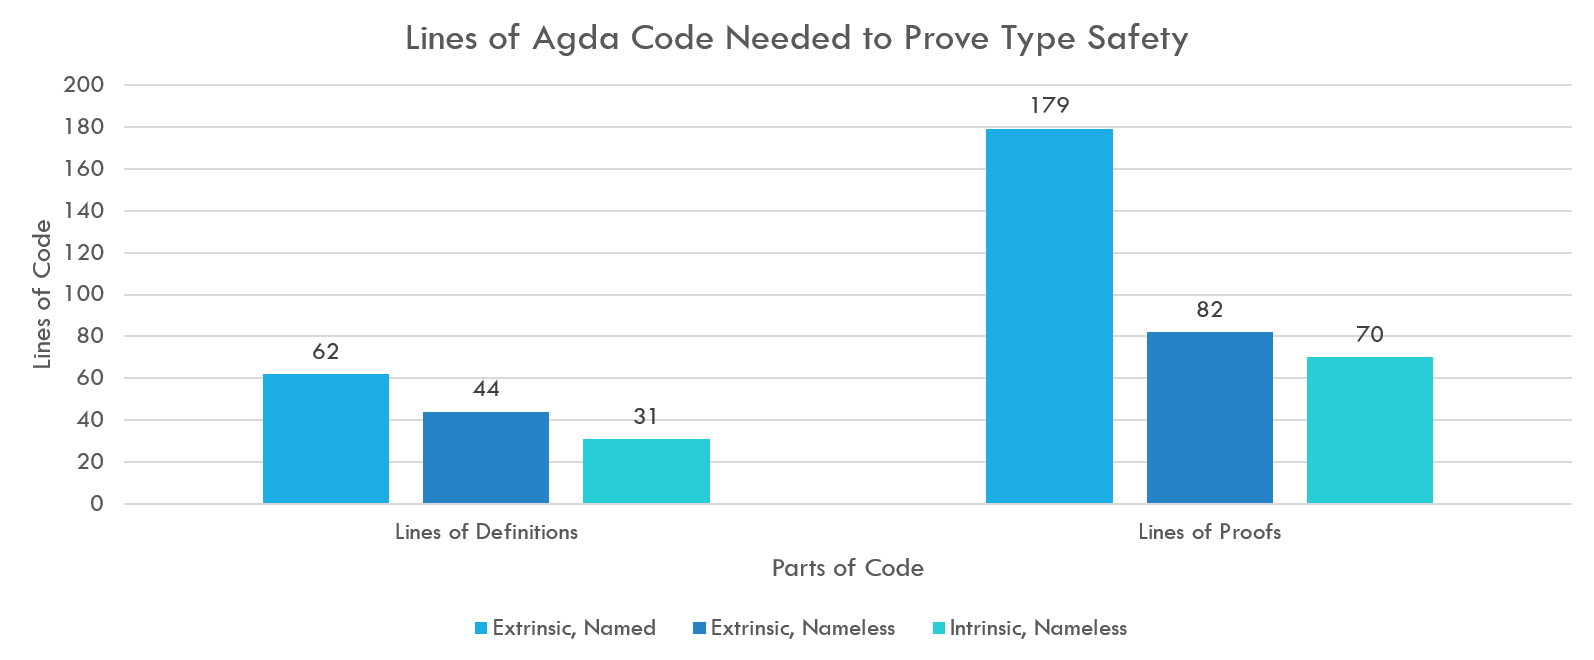
\includegraphics[scale=0.6]{results}
\caption{Number of lines of Agda code needed to prove type safety.}
\label{fig:results}
\end{figure}
Note that we are not counting the definitions and proofs of standard library tools, such as sum types and product types, equivalence relations and their associated properties, and general deduction strategies, such as \textit{ex falso quodlibet}. The results are shown in Figure \ref{fig:results}. We found that using named variables drastically increased the number of lines of code needed to prove type safety for both definition and proof. We also found that using extrinsic typing requires more lines of definition proof than using intrinsic typing, although the difference is not as extreme. 

\section{Discussion}

\subsection{Named Variables vs. Nameless Variables}
When going from using named variables to using nameless variables, we were able to avoid defining and proving many results related to variable shadowing when performing substitution. For example, performing the following substitution:
\begin{align*}
[ \text{true} / x ] ((\lambda x : \text{bool} . x)\;x)
\end{align*}
yields:
\begin{align*}
(\lambda x : \text{bool} . x)\;\text{true}
\end{align*}
and not:
\begin{align*}
(\lambda x : \text{bool} . \text{true})\;\text{true}
\end{align*}
This is because, by convention, we interpret the $x$ in the body to refer to the inner binding. We refer to this phenomenon as variable shadowing. Therefore, we need to expend additional effort to account for this in our proofs. However, for nameless terms, ensuring that the corresponding substitution:
\begin{align*}
[ \text{true} / \langle 0 \rangle ] ((\lambda \underline{\;\;\;} : \text{bool} . \langle 0 \rangle)\;\langle 0 \rangle)
\end{align*}
yields:
\begin{align*}
(\lambda \underline{\;\;\;} : \text{bool} . \langle 0 \rangle)\;\text{true}
\end{align*}
is much simpler because we know that in the function body, we should be replacing instances of $\langle 1 \rangle$, since a new variable has been bound when entering the body of the function.

Furthermore, the current proof of type safety for $\lambda^{\to}$ with named variables does not attempt to address the issue of variable capture. As mentioned before, in a call-by-value order of evaluation, one can exclude functions with unbound variables from the definition of values, which implies that unbound variables will never be captured during substitution. However, if we were to change the order of evaluation to full $\beta$-reduction, which will also attempt to perform substitution on all application expressions, the current proof of type safety for $\lambda^{\to}$ with named variables will not go through. In contrast, type safety proofs for $\lambda^{\to}$ with nameless variables is robust to this change because variable are never referenced ambiguously.

However, we find that using named variables aids in the human interpretability of terms of $\lambda^{\to}$. To interpret a term that uses de Brujin indices for variables, one must continuously count backward the number of steps equal to the indices to determine the semantics of the variables, which can easily become unwieldy in highly nested terms. For example, most would agree that:
\begin{align*}
\lambda x : \text{bool} \to \text{bool}. \lambda y : \text{bool}. (\lambda z : \text{bool}. x\;z)\;((\lambda v : \text{bool}.\lambda w : \text{bool}.x\;v) \;y \;y)
\end{align*}
is much more interpretable than:
\begin{align*}
\lambda \underline{\;\;\;} : \text{bool} \to \text{bool}. \lambda \underline{\;\;\;} : \text{bool}. (\lambda \underline{\;\;\;} : \text{bool}. \langle 2 \rangle\;\langle 0 \rangle)\;((\lambda \underline{\;\;\;} : \text{bool}.\lambda \underline{\;\;\;} : \text{bool}.\langle 3 \rangle\;\langle 1 \rangle) \;\langle 0 \rangle \;\langle 0 \rangle)
\end{align*}
One would imagine that interpreting the $\langle 0 \rangle$ at the end of the expression to be the second bound variable in the expression would require more effort than matching the name $y$ in the example with names. Therefore, we can conclude that while named variables make proofs about programming languages more difficult, they still provide other important benefits that go beyond proofs.

\subsection{Extrinsic Typing vs. Intrinsic Typing}
On the other hand, when going from extrinsic typing to intrinsic typing, we see that we save having to define an external \texttt{Type-Proof} data type, as well as save a few more lines of definition in collapsing functions that would otherwise perform analogous operations on terms and typing judgments. The main source of savings for lines of proofs comes from not having to prove the Preservation theorem and its dependencies, such as the Uniqueness of Types theorem, which states that in any context, a term has at most one type. 

However, similar to the case of named variables vs. nameless variables, we see that having extrinsic typing allows terms to be written down and interpreted much more easily. At the cost of being able to write down ill-typed terms, we greatly reduce the amount of effort it takes to represent a term in the language. Furthermore, the task of determining whether a term is well typed or not can be done algorithmically, using methods such as Robinson's unification algorithm \cite{robinson}. Therefore, as a practical matter, it is more convenient to let human programmers write down the terms in the language, and to use a machine to derive the proper typing judgment for those terms. 

\section{Conclusion and Future Work}

In this project, we studied three different formalizations of the simply typed lambda calculus and compared how they affected the structure and difficulty of the respective proofs of type safety. We found that type safety can be proven much more easily in a language that uses intrinsic typing and nameless variables, and while having an extrinsic typing mechanism does not complicate type safety proofs by much, using named variable can significantly increase the amount of work necessary. However, from a practical point of view, it is much better to program in a language that uses variable names and that does not require one to provide proofs of well-typedness as part of the syntax. 

One possible direction to explore is to use some of the more recently developed techniques in type theory, such as \textbf{higher inductive types}, to formalize a version of $\lambda^{\to}$ that allows for named variables in the language while simultaneously avoiding many of the problems associated with variable names. A higher inductive type allows us not only to define constructors for a given type, but also to define artificial equivalences between terms of that type. For example, we can use a higher inductive type to define the terms of $\lambda^{\to}$, and then define all terms that differ by a renaming of a bound variable (often called an $\alpha$-conversion) to be equivalent (i.e. $\alpha$-equivalent). This will resolve the issue of variable capture during substitution, as we can simply use $\alpha$-equivalence to convert the problematic terms to equivalent forms that have no variable name collision. Furthermore, since such a conversion is done in the context of an equivalence, proofs about these conversions will hopefully turn out to be relatively short because we are able to leverage properties of equivalences, such as symmetry, transitivity, congruence, etc., which we are able to use directly.

Overall, there is much more to be explored in the realm of formalization of type safety proofs. We hope to continue to explore this more.


\bibliography{bib}
\bibliographystyle{plain}

\section*{Appendix}
Detailed definitions and proofs of type safety in Agda for the three formalizations studied in this project can be found online here:
\url{https://github.com/coolfan/cos-iw-s2019}. Please look in the following files:
\begin{enumerate}
	\item \texttt{stlc-extrinsic.agda}: Extrinsically typed $\lambda^{\to}$ with named variables
	\item \texttt{stlc.agda}: Extrinsically typed $\lambda^{\to}$ with nameless variables
	\item \texttt{stlc-intrinsic.agda}: Intrinsically typed $\lambda^{\to}$ with nameless variables
\end{enumerate}

\end{document}